% -*- mode: fundamental -*-

% Document describing microarchitecture of:
% Simulation top-level, synthesizable SoC, for Piccolo, Flute, Toooba etc.
% and cores and CPUs for Piccolo and Flute.
% Begun by Nikhil, January 18, 2020

\documentclass[11pt]{book}

% ================================================================
\usepackage[latin1]{inputenc}
\usepackage[T1]{fontenc}
\usepackage{latexsym}
\usepackage{makeidx}
\usepackage{alltt}
\usepackage{verbatim}
\usepackage{fancyvrb}
% \usepackage{moreverb}
\usepackage{ae}
\usepackage{aecompl}
%newly added
\usepackage{subcaption}
\usepackage{multirow}
\usepackage{hhline}
\usepackage{textcomp}

  \usepackage[pdftex,colorlinks=true,bookmarksopen, pdfstartview=FitH,
              linkcolor=blue, citecolor=blue, urlcolor=blue]{hyperref}
  \pdfcompresslevel=9
  \usepackage[pdftex]{graphicx}

% ================================================================

% HORIZONTAL MARGINS
% Left margin, odd pages: 1.25 inch (0.25 + 1)
\setlength{\oddsidemargin}{0.25in}
% Left margin, even pages: 1.25 inch (0 + 1)
\setlength{\evensidemargin}{0.25in}
% Text width 6 inch (so other margin is 1.25 inch).
\setlength{\textwidth}{6in}
% ----------------
% VERTICAL MARGINS
% Top margin 0.5 inch (-0.5 + 1)
\setlength{\topmargin}{-0.5in}
% Head height 0.25 inch (where page headers go)
\setlength{\headheight}{0.25in}
% Head separation 0.25 inch (between header and top line of text)
\setlength{\headsep}{0.25in}
% Text height 9 inch (so bottom margin 1 in)
\setlength{\textheight}{9in}
% ----------------
% PARAGRAPH INDENTATION
\setlength{\parindent}{0in}
% SPACE BETWEEN PARAGRAPHS
\setlength{\parskip}{\medskipamount}
% ----------------
% STRUTS
% HORIZONTAL STRUT.  One argument (width).
\newcommand{\hstrut}[1]{\hspace*{#1}}
% VERTICAL STRUT. Two arguments (offset from baseline, height).
\newcommand{\vstrut}[2]{\rule[#1]{0in}{#2}}
% ----------------
% HORIZONTAL LINE ACROSS PAGE:
\newcommand{\hdivider}{\noindent\mbox{}\hrulefill\mbox{}} 
% ----------------
% EMPTY BOXES OF VARIOUS WIDTHS, FOR INDENTATION
\newcommand{\hm}{\hspace*{1em}}
\newcommand{\hmm}{\hspace*{2em}}
\newcommand{\hmmm}{\hspace*{3em}}
\newcommand{\hmmmm}{\hspace*{4em}}
% ----------------
% VARIOUS CONVENIENT WIDTHS RELATIVE TO THE TEXT WIDTH, FOR BOXES.
\newlength{\hlessmm}
\setlength{\hlessmm}{\textwidth}
\addtolength{\hlessmm}{-2em}

\newlength{\hlessmmmm}
\setlength{\hlessmmmm}{\textwidth}
\addtolength{\hlessmmmm}{-4em}
% ----------------
% ``TIGHTLIST'' ENVIRONMENT (no para space betwee items, small indent)
\newenvironment{tightlist}%
{\begin{list}{$\bullet$}{%
    \setlength{\topsep}{0in}
    \setlength{\partopsep}{0in}
    \setlength{\itemsep}{0in}
    \setlength{\parsep}{0in}
    \setlength{\leftmargin}{1.5em}
    \setlength{\rightmargin}{0in}
    \setlength{\itemindent}{0in}
}
}%
{\end{list}
}
% ----------------
% ITALICISE WORDS
\newcommand{\ie}{\emph{i.e.,}}
\newcommand{\eg}{\emph{e.g.,}}
\newcommand{\Eg}{\emph{E.g.,}}
\newcommand{\etc}{\emph{etc.}}
\newcommand{\via}{\emph{via}}
\newcommand{\vs}{\emph{vs.}}
% ----------------
% CODE FONT (e.g. {\cf x := 0}).
\newcommand{\cf}{\footnotesize\tt}
% ----------------
% \FIT = footnotesize italics
\newcommand{\fit}{\footnotesize\it}
% ----------------
% KEYWORDS
\newcommand{\kw}[1]{{\bf #1}}
% ----------------
% INLINE CODE EXPRESSIONS
\newcommand{\inlcode}[1]{``\mbox{\cf #1}''}

% ----------------------------------------------------------------
% ----------------------------------------------------------------
% HERE BEGINS THE DOCUMENT

\newcommand{\copyrightnotice}{\textcopyright 2020 Bluespec, Inc.}
\newcommand{\BSV}{BSV}
\newcommand{\BH}{Bluespec~Haskell}

% ================================================================

\begin{document}

% ================================================================
% Front matter

\pagestyle{empty}

\begin{center}

\vspace*{1in}

{\LARGE\bf Microarchitecture overview of RISC-V Processors}

\vspace{1ex}

{\LARGE\bf (Free and  Open-Source)}

\vspace{1ex}

{\LARGE\bf from Bluespec, Inc.}

\vspace{1ex}

{\Large\bf at https://github.com/bluespec/Piccolo, Flute, Toooba, ...}

\vspace{0.5in}

{\Large \emph{Rishiyur S. Nikhil}}

{\Large Bluespec, Inc.} \\

\vspace*{3in}

\textcopyright{} 2020 Rishiyur S. Nikhil

\vspace{0.5in}

Version: January 20, 2020

\end{center}

% ================================================================
% PREFACE AND ACKNOWLEDGEMENTS

\newpage

\pagenumbering{roman}
\setcounter{page}{2}

\vspace*{2in}

\noindent
\subsection*{Acknowledgements}

... \emph{To be written} ...

% ================================================================
% TABLE OF CONTENTS

\pagestyle{myheadings}

\markboth{CONTENTS}{}

{\small

\tableofcontents

}

% ****************************************************************

\newpage

\chapter{Introduction, and Simulation Top-level}

\markboth{Intro and Simulation/System Top-level}{\copyrightnotice}

\renewcommand{\thepage}{\arabic{chapter}-\arabic{page}}
\setcounter{page}{1}
% \renewcommand{\thepage}{\arabic{page}}

\label{ch_Intro}

% ================================================================

\section{Introduction}

Bluespec, Inc. provides three free, open-source RISC-V processors on
GitHub (with more to come in the future).

\begin{itemize}

\item {\bf Piccolo}: simple 3-stage, in-order. \\
\hmm {\tt https://github.com/bluespec/Piccolo}

\item {\bf Flute}: simple 5-stage, in-order, some
control-flow speculation and branch prediction. \\
\hmm {\tt https://github.com/bluespec/Flute}

\item {\bf Toooba}: aggressive superscalar, out-of-order, agressive
speculation and branch prediction. \\
\hmm {\tt https://github.com/bluespec/Toooba}

\end{itemize}

All three are Linux-capable (can be built for RV64IMAFD with Machine
and Supervisor privilege levels; Sv39 virtual memory; and external,
software and timer interrupts).

Piccolo and Flute are highly parameterized and can also be built with
smaller capabilities (e.g., embedded, IoT).  In particular, you can
choose any of the following ISA options:

\begin{tightlist}

\item RV32I or RV64I
\item M (integer multiply/divide)
\item A (atomics)
\item F (single-precision floating point)
\item D (double-precision floating point)
\item C (compressed instructions)
\item S (Supervisor privilege level), with Sv32 virtual memory for
RV32 and Sv39 or Sv48 virtual memory for RV64

\item U (User privilege level)

\end{tightlist}

Piccolo and Flute have separate instruction and data memory channels,
with L1 caches where you can choose cache sizes and organization.

Toooba is RV64IMAFDC with Sv39 virtual memory, and multicore.  It has
many parameter choices such as degree of superscalarity, L1 cache size
and organization, L2 cache size and organization, reorder buffer size,
number of arithmetic, floating point and memory pipelines, size of
store buffers, memory model, number of cores, etc.

% ----------------------------------------------------------------

\subsection{Purpose of this document/target audience(s)}

This document is intended for people trying to use the pre-generated
Verilogs in the repositories, and for people trying to understand the
BSV source code in the repositories with a view to regenerating the
Verilogs, perhaps with custom changes.  It is intended to provide
top-level context for the code and code structure so that you can
navigate the directories and read the code and/or understand how to
use the pre-generated Verilog.

Here are several possible use models for the code in these repos:

\begin{itemize}

\item Take the pre-generated Verilogs for the RISC-V CPUs, as-is, for
use in the user's own SoC.  The SoC provided in these repos allows
developing and debugging software immediately even if the user's SoC
is not yet ready.

\item Choose different parameters (relative to the pre-generated
Verilogs) for the CPUs, and regenerate the Verilogs, for use in the
user's own SoC.  E.g., choose a different set of RISC-V options
(RV32/RV64, A, M, F, D, C, with/without Supervisor and virtual memory,
...)

\item Modify the BSV code for the CPUs for the user's customizations,
and re-generate the Verilogs.  E.g., add new custom instructions.

\item Use the system here as a ``socket'' to plug in the user's own
RISC-V CPU implementation, giving the user a system that can run
software out of the box with full debugging support, even if the
user's SoC is not yet ready.

\item Use the CPU and SoC here as is, just adding extra AXI4 ports on
the system interconnect to connect the user's own memory-mapped
accelerator.  The user can develop software for the accelerator and
test it immediately, with full debugger control.

\end{itemize}

This document does not attempt to explain the BSV High Level Hardware
Design Language.  For that, please refer to language manuals and
tutorials at {\cf https://github.com/BSVLang/Main/}.

This document does not attempt to do a detailed code explanation of
the BSV code in the repositories.  Rather, this document is only meant
to provide you high level context and structure so that you can, on
your own, easily navigate through the directories and files.

% ================================================================

\section{Common ``system'' for all three processors}

The GitHub repositories for Piccolo, Flute and Toooba include a common
``system'' environment for the processors so that they can execute
RISC-V binaries out of the box, using Verilog simulation.  Most of
this system is also synthesizable for FPGA or ASIC.

Fig.~\ref{Fig_100_Top_HW_Side} illustrates the structure of the common
top-level system.
\begin{figure}[htbp]
  \centerline{
\includegraphics[height=2in,angle=0]{Figures/Fig_100_Top_HW_Side.png}}
  \caption{\label{Fig_100_Top_HW_Side}The top-level of the module hierarchy of the system.}
\end{figure}

\emph{Notation in figure}: Nested rectangles indicate module
hierarchy.  Here, module {\cf mkTop\_HW\_Side} instantiates module
{\cf mkSoC\_Top} with instance-name {\cf soc\_top} and instantiates
module {\cf mkMem\_Model} with instance-name {\cf mem\_model}.  Module
{\cf mkSoC\_Top}, in turn, instantiates module {\cf mkCore} with
instance-name {\cf core}.

Fig.~\ref{Fig_200_SoC_Top} expands the {\cf mkSoC\_Top} module for more detail.
\begin{figure}[htbp]
  \centerline{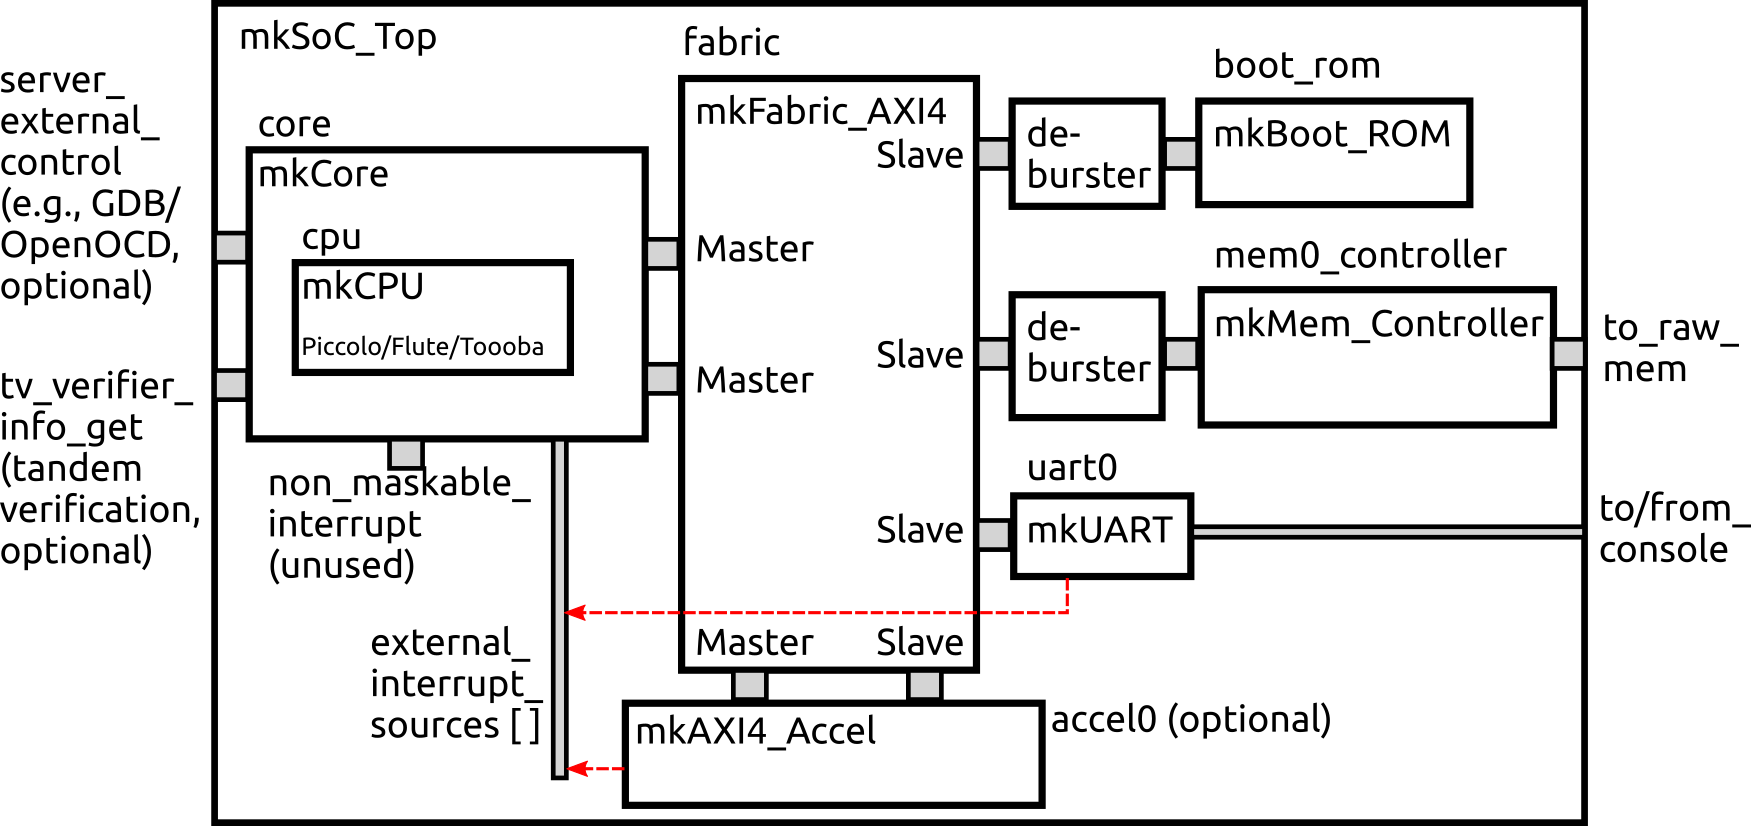
\includegraphics[height=2.5in,angle=0]{Figures/Fig_200_SoC_Top.png}}
  \caption{\label{Fig_200_SoC_Top}The common SoC structure shared in all repos.}
\end{figure}

At the center is an AXI4 fabric (interconnection network) that
connects a parameterizable number of master ports to a
parameterizable number of slave ports.  Two of the master ports are
used by {\cf mkCore} inside which is the Piccolo/Flute/Toooba CPU.
The slave ports are connected to a Boot ROM, a memory and a UART, and
optionally to one or more memory-mapped accelerators.

The core can optionally be controlled by an external debugger (e.g.,
GDB and OpenOCD).  It can optionally send out a detailed
instruction-by-instruction trace for ``Tandem Verification'' with a
golden reference model of a RISC-V CPU.  It can accept external
interrupts from I/O devices.  The two master ports into the fabric are
peers and can be used in different ways.  In Piccolo and Flute, one
master port is used for all instruction traffic and the other is used
for all data (memory and I/O traffic).  In Toooba, one master is used
for all memory traffic (instruction and data) and the other is used
for all I/O traffic.

The Boot ROM and Memory-Controller modules do not handle AXI4 bursts;
the ``deburster'' modules convert burst requests from and responses to
the fabric into individual request/responses to the modules behind
them.  The Memory Controller has an interface taken all the way out of
{\cf mkSoC\_Top} to an external DRAM controller of 256-bits of
512-bits width.

The UART has an interface taken all the way out of {\cf mkSoC\_Top}
streaming bytes in and out.

The core and the CPU have a ``non-maskable interrupt'' input interface
that is not used in this SoC (in a real chip, they might be connected
to sensors signaling power failure, temperature overheating, etc.).

There are two versions of {\cf mkCore}, one shared by Piccolo and
Flute, and the other for Toooba.  The former is described in more
detail in Ch.~\ref{ch_mkCore_Piccolo_Flute}, and the latter in
Ch.~\ref{ch_mkCore_Toooba}.  In addition to the CPU pipelines
themselves, the cores include:

\begin{tightlist}

\item I- and D-caches;

\item TLBs and virtual-memory management (including hardware page-table walkers);

\item a set of ``near-memory I/O'' components such as a memory-mapped
real-time timer, and memory-mapped software-interrupt location;

\item a PLIC (Platform Level Interrupt Controller);

\item an optional Debug Module;

\item and an optional Tandem Verification output trace encoder.

\end{tightlist}

The CPU pipelines themselves are described separately for Piccolo in
Ch.~\ref{ch_Piccolo}, Flute in Ch.~\ref{ch_Flute}, and for Toooba in
Ch.~\ref{ch_Toooba}.

Optionally, one can have one or more memory-mapped accelerators
connected to extra master and slave ports.  Typically, a memory-mapped
accelerator is programmed/configured and ``started'' by the processor
using writes through a fabric slave port.  The accelerator, once
running, accesses memory directly using reads and writes through a
fabric master port.  Completion of the acceleration task is detected
by the processor either by polling (reads) on the slave port, or by
receiving an interrupt from the accelerator.

% ================================================================

\section{Common directory organization}

In general, a module {\cf mkFoo} can be found in a file {\cf Foo.bsv}.

All the repositories also follow a common directory organization:

\begin{itemize}

\item The directory {\cf src\_Core/} contains {\cf mkCore} (in {\cf
file Core.bsv}) and everything inside it, including the CPU pipelines,
L1 caches, PLIC (Platform Level Interrupt Controller), Debug Module,
and Tandem Verification trace generator.

\item The directory {\cf src\_Testbench/SoC/} contains {\cf
mkSoC\_Top} and other SoC components.

\item The {\cf src\_bsc\_lib\_RTL} contains copies of a few Verilog
library files used by the Bluespec \emph{bsc} compiler, and can be
treated here as black boxes.

\item The {\cf src\_SSITH\_P1/P2/P3} directories can be ignored; they
contain different wrappers of {\cf src\_Core} intended for the DARPA
SSITH project and are not otherwise relevant.

\end{itemize}

Linux/Unix users will be familiar with the standard 'find', which is
useful to locate a file with a given name in the directory tree below
the current directory:
\begin{Verbatim}[frame=single]
   $ find . -name <filename>
\end{Verbatim}
Similarly, the standard program 'grep' is useful to locate a file
containing a specific substring in the directory tree below the
current directory:
\begin{Verbatim}[frame=single]
   $ grep -Rn <string>  .                # Case sensiitive
   $ grep -iRn <string>  .               # Case insensitive
\end{Verbatim}

% ================================================================

\section{Pre-generated Verilogs, regenerating them, and generating new configurations}

\label{sec_pre_gen_Verilog}

The repositories contain pre-generated Verilog for certain
configurations as subdirectories of the {\cf builds/} directory.  For
example, in the Piccolo repository, the directory
\begin{Verbatim}[frame=single]
    builds/RV64ACFDIMSU_Piccolo_verilator
\end{Verbatim}
is for building Piccolo for RV64I with ISA options ACDFIMSU for
verilator.  The sub-directory {\cf Verilog\_RTL/} has the
pre-generated Verilog for this.

If you have an installation of the Bluespec BSV \emph{bsc} compiler,
you can re-generate the Verilogs, or build a Bluesim simulation, or
generate other configurations (see the README in the repo for how to
compile and build).

% ================================================================

\section{Using just the core in your own designs}

\label{sec_mkCore}

In Fig.~\ref{Fig_100_Top_HW_Side}, {\cf mkCore} is the basic core: CPU
pipeline, L1 caches, PLIC (Platform Level Interrupt Controller), and
optional Debug Module and Tandem Verification trace generator.

For Piccolo and Flute, in the pre-generated Verilog directories (see
Sec.~\ref{sec_pre_gen_Verilog}), the code is in file {\cf mkCore.v} and
other Verilog files representing the module hierarchy below it.

For Toooba, in the pre-generated Verilog directories, the code is the
file {\cf mkCoreW.v} and other Verilog Verilog files representing the
module hierarchy below it.

The interface of the core module is the same for all three CPUs:

\begin{itemize}

\item {\cf CLK} and {\cf RST\_N} are the clock and reset inputs.

\item The buses named {\cf cpu\_imem\_master\_*} are an AXI4 master interface.

\item The buses named {\cf cpu\_dmem\_master\_*} are an AXI4 master interface.

\item The following buses are useful in simulation for debugging:
  \begin{tightlist}
    \item {\cf set\_verbosity\_verbosity}
    \item {\cf set\_verbosity\_logdelay}
    \item {\cf EN\_set\_verbosity}
    \item {\cf RDY\_set\_verbosity}
  \end{tightlist}
  When the {\cf RDY} output is high, the enviroment can assert the
  {\cf EN} input and drive the other two inputs, setting the cycle
  delay after which the verbosity should change, and the verbosity
  value to which it should change.  Verbosity of 1 will print an
  instruction trace; higher values will print more detail from the CPU
  pipeline.

\item The 'reset' signals are for a 'soft' reset of the core to its
  initial state (the same state as after the electrical reset {\cf
  RST\_N}).  They come in two groups representing a request/response
  protocol, since a full reset of the core can take multiple cycles.

  When output {\cf RDY\_cpu\_reset\_server\_request\_put} is 1, the
  environment can request a reset by asserting {\cf
  EN\_cpu\_reset\_server\_request\_put} and driving a 0 or 1 on {\cf
  cpu\_reset\_server\_request\_put}.  Driving a 1 specifies that,
  after the reset, the CPU should come up running (the normal case).
  Driving a 0 specifies that the CPU should come up halted in Debug
  Mode, waiting for commands from an external debugger.

  When output {\cf RDY\_cpu\_reset\_server\_response\_get} is 1, it
  indicates that the core has reset itself.  The environment can read {\cf
  cpu\_reset\_server\_response\_get} to see if the core is running (1)
  or halted (0).  The environment can assert {\cf
  EN\_cpu\_reset\_server\_response\_get} to acknowledge to the core
  that it has observed this information.

\item The core contains a standard RISC-V PLIC (Platform Level
  Interrupt Controller) supporting 16 external interrupts at the ``m''
  (machine) privilege level.  These are the 16 input signals of the form:
{\cf core\_external\_interrupt\_sources\_$j$\_m\_interrupt\_req\_set\_not\_clear}

\item The core supports a \emph{non-maskable interrupt} on the input
  signal {\cf nmi\_req\_set\_not\_clear}, intended for very urgent
  interrupts such as power failures, thermal overload, etc.

\end{itemize}

% ================================================================

\section{Using SoC in your own designs, with these or other cores}

In Fig.~\ref{Fig_100_Top_HW_Side}, {\cf mkSoC\_Top} is a basic SoC
(System-on-a-chip).

In all the repositories, in the pre-generated Verilog directories (see
Sec.~\ref{sec_pre_gen_Verilog}), the code is in file {\cf mkSoC\_Top.v}
and other Verilog files representing the module hierarchy below it.
The SoC contains:

\begin{tightlist}

\item The RISC-V core, described in the previous
Sec.~\ref{sec_mkCore}, is in file {\cf mkCore.v}.  You can use this {\cf
mkCore.v} or substitute your own core with the same Verilog interface.

\item An AXI4 crossbar fabric (file {\cf mkFabric\_AXI4.v}).

\item A boot ROM (file {\cf mkBoot\_Rom.v}) with an AXI4 interface (without burst support).

\item A memory controller, front end for a DRAM controller (file {\cf
mkMem\_Controller}) with and AXI4 interface (without burst support).

\item An AXI4 to AXI4 slave adapter, instantiated twice, once for the
Boot ROM and once for the memory controller (file {\cf
mkAXI4\_Deburster\_A.v}), so that they can support burst AXI4
requests.

\item A synthesized model of an NS16550 UART (file {\cf mkUART.v}).

\end{tightlist}

% ****************************************************************

\newpage

\chapter{Common {\tt mkCore} structure for Piccolo and Flute}

\markboth{mkCore: Piccolo and Flute}{\copyrightnotice}

\renewcommand{\thepage}{\arabic{chapter}-\arabic{page}}
\setcounter{page}{1}
% \renewcommand{\thepage}{\arabic{page}}

\label{ch_mkCore_Piccolo_Flute}

The {\cf mkCore} module for Piccolo and Flute in Fig.~\ref{Fig_200_SoC_Top} is shown in
more detail in Fig.~\ref{Fig_300_mkCore}.
\begin{figure}[htbp]
  \centerline{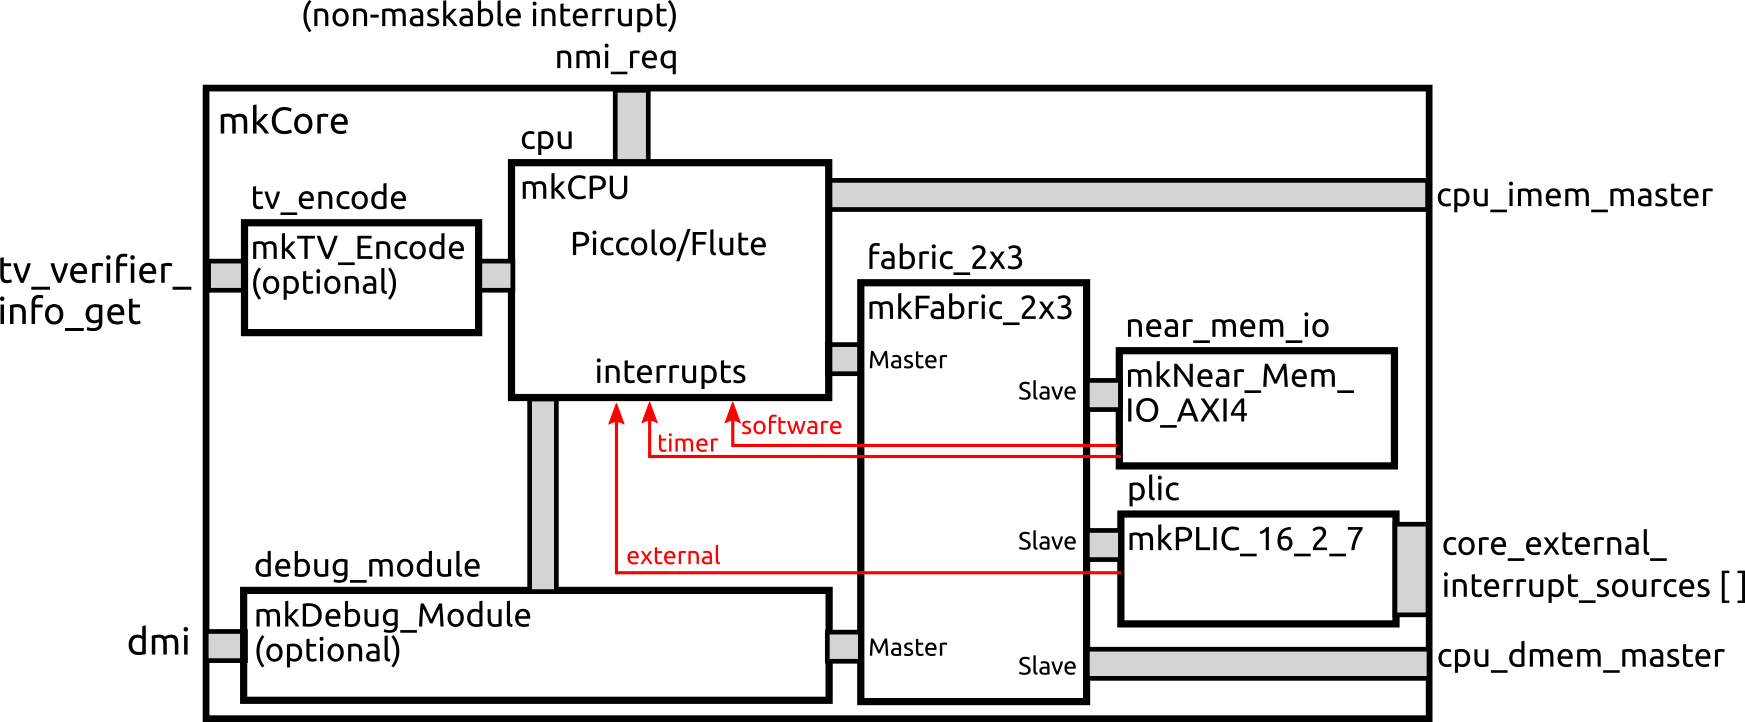
\includegraphics[height=2.5in,angle=0]{Figures/Fig_300_mkCore.png}}
  \caption{\label{Fig_300_mkCore}The common mkCore for Piccolo and Flute.}
\end{figure}

The {\cf mkCPU} module is the Piccolo or Flute CPU with L1 caches and
MMUs.  The interface is identical for Piccolo and Flute.  In the
figure, on the right, it has two AXI4 interfaces.  One of them goes
straight out to the {\cf mkCore} interface for instruction access as
the {\cf cpu\_imem\_master} interface; this is an AXI4 master.  The
other, for data memory and I/O access, is also an AXI4 master, but
it connects to a 2x3 interconnect fabric.  The 2x3 fabric has three
AXI4 slaves:
\begin{tightlist}

\item {\cf mkNear\_Mem\_IO\_AXI4} contains ``nearby'' memory-mapped
locations, such as the RISC-V standard real-time timer (MTIME),
timer-compare (MTIMECMP) and software-interrupt (MSIP).  Interrupts
generated from these, in turn, are connected back to mkCPU (red
arrows).

\item {\cf mkPLIC}, a standard RISC-V Platform Level Interrupt
Controller.  It accepts a vector of external interrupt sources and
arbitrates them, finally feeding the winning interrupt(s) into {\cf
mkCPU}.

\item A direct connection out to the main system interconnect, {\cf
cpu\_dmem\_master} for all other data memory and I/O device access.

\end{tightlist}

% ================================================================

\section{Optional Debug Module}

\label{sec_Debug_Module}

An optional RISC-V standard Debug Module {\cf mkDebug\_Module} has
connections into {\cf mkCPU} for run-control (halt, resume) and access
to GPRs, FPRs and CSRs.  It is also a second master on the {\cf
mkFabric\_2x3} so that it can access all memory and I/O devices.  On
the left of {\cf mkDebug\_Module} has a standard ``DMI'' (Debug Module
Interface) which is a memory-like read/write interface by which an
external debugger interacts with the Debug Module.  A typical
setup would be:

\begin{quote}
GDB $\Longleftrightarrow$ OpenOCD $\Longleftrightarrow$ JTAG transport $\Longleftrightarrow$ DMI
\end{quote}

Source code in the {\cf src\_SSITH\_Pn/src\_BSV/} directory is
available for the JTAG connection to OpenOCD.

The Debug Module gives GDB full control over the RISC-V CPU, including
$\uparrow$C (halt a running program); setting/removing breakpoints;
reading and writing memory, GPRs, FPRs and CSRs (including the PC);
single-stepping; resetting the CPU; and resetting the system.

% ================================================================

\section{Optional Tandem Verification Trace Generation}

\label{sec_Tandem_Verifier}

The optional {\cf mkTV\_Encode} module sends out an
instruction-by-instruction trace to an external recorder/analyzer.
Information associated with each instruction includes the PC, the
instruction itself, updates to GPRs/FPRs/CSRs, updates to memory and
the next PC.  For memory instructions it also includes the effective
address.

This output trace can be compared with an expected trace on a ``golden
reference model''; a divergence typically reveals a bug in the
hardware implementation for some particular kind of instruction.

% ****************************************************************

\newpage

\chapter{Piccolo}

\markboth{Piccolo}{\copyrightnotice}

\renewcommand{\thepage}{\arabic{chapter}-\arabic{page}}
\setcounter{page}{1}
% \renewcommand{\thepage}{\arabic{page}}

\label{ch_Piccolo}

% ================================================================

... \emph{To be written} ...

% ****************************************************************

\newpage

\chapter{Flute}

\markboth{Flute}{\copyrightnotice}

\renewcommand{\thepage}{\arabic{chapter}-\arabic{page}}
\setcounter{page}{1}
% \renewcommand{\thepage}{\arabic{page}}

\label{ch_Flute}

% ================================================================

Fig.~\ref{Fig_500_mkCPU_Flute} shows the major module structure
inside {\cf mkCPU} for Flute.
\begin{figure}[htbp]
  \centerline{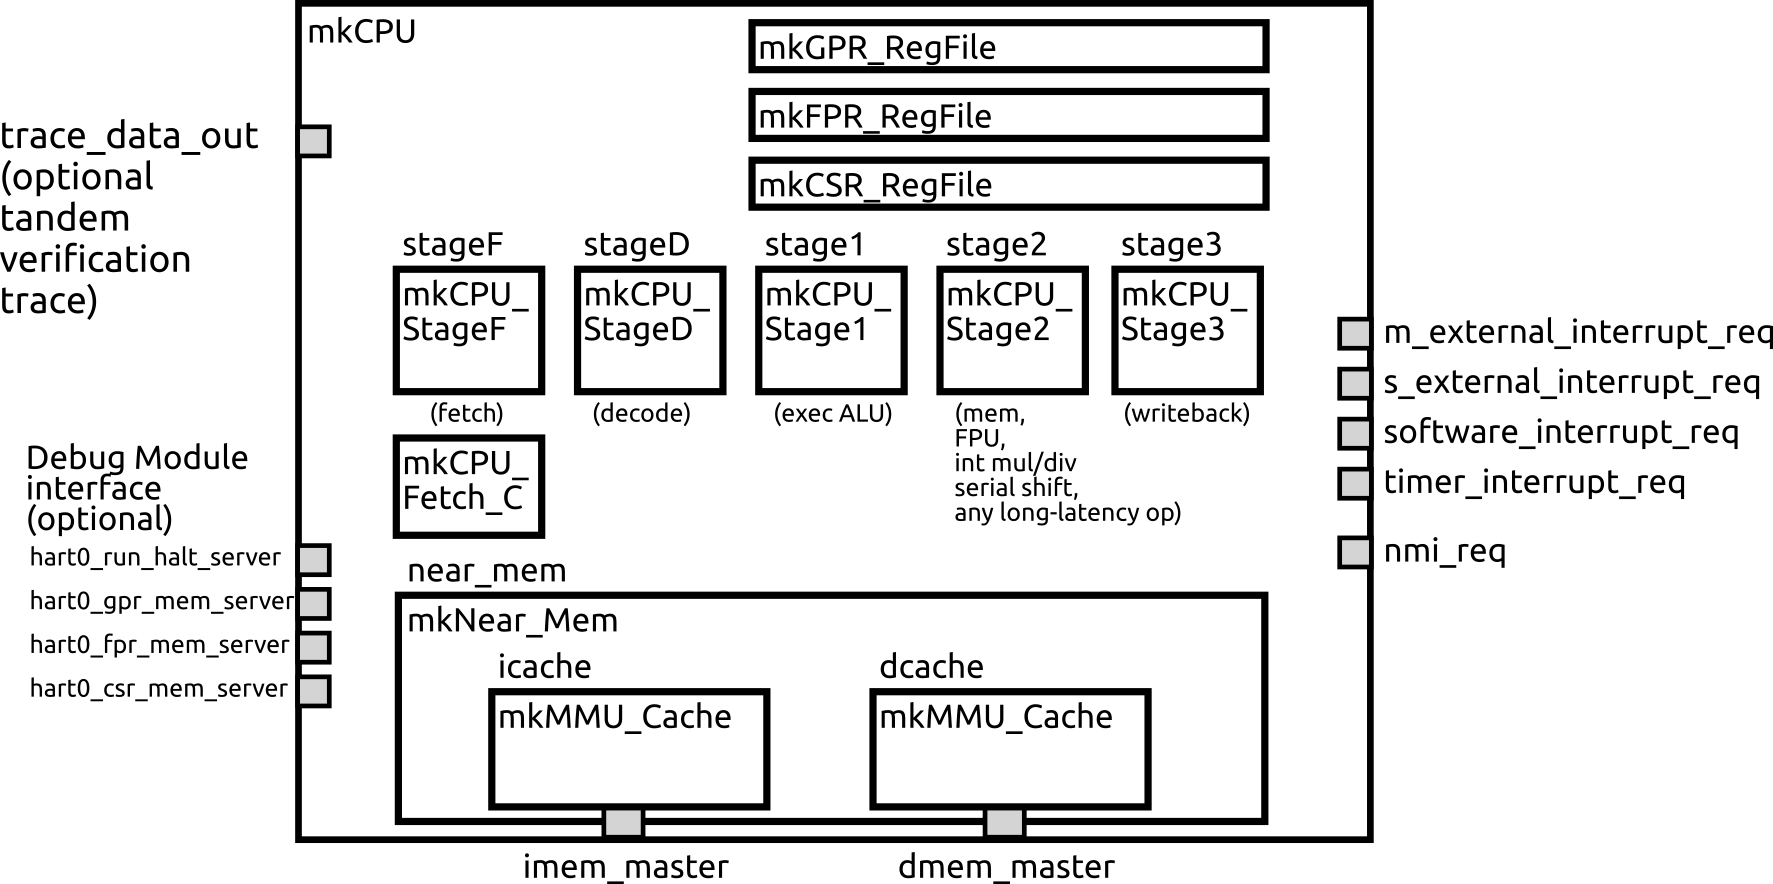
\includegraphics[height=3in,angle=0]{Figures/Fig_500_mkCPU_Flute.png}}
  \caption{\label{Fig_500_mkCPU_Flute}Flute module structure.}
\end{figure}
At the heart is a 5-stage pipeline embodied in the following modules:
\begin{tightlist}

\item {\cf stageF}, an instantiation of {\cf mkCPU\_StageF}. This is
the Fetch stage.  The Fetch stage includes a branch predictor (branch
target buffer and return-address stack).  If the CPU is built with the
RISC-V C extension (Compressed instructions), an additional module
{\cf mkCPU\_Fetch\_C} is interposed in front of the instruction-memory
that decides whether the next instruction delivered is a C instruction
or a normal RV32/RV64 instruction.

\item {\cf stageD}, an instantiation of {\cf mkCPU\_StageD}. This is
the Decode stage.  If the CPU is built with the RISC-V C extension
(compressed instructions), the decode stage includes expansion of C
instructions to their normal RV32/RV64 counterparts.

\item {\cf stage1}, an instantiation of {\cf mkCPU\_Stage1}. This is
the Execute stage for all single-cycle ALU operations.  Conditional
branches and jumps are resolved here, and results are fed back to
StageF to redirect on mispredictions and to train the Branch
Predictor.

\item {\cf stage2}, an instantiation of {\cf mkCPU\_Stage2}. This
stage has parallel paths for all potentially long-latency operations
including memory access (load, store, atomics), floating point (RISC-V
F and D extensions), integer multiply/divide (RISC-V M extension),
optional serial shifter (instead of a barrel shifter in Stage 1), etc.

\item {\cf stage3}, an instantiation of {\cf mkCPU\_Stage3}, the
writeback stage where final values are written back to the GPR and FPR
register files.

\end{tightlist}
The reason for the somewhat unusual naming scheme (instead of stages
1..5), is because of the code-sharing structure with Piccolo, a
3-stage pipeline.  Piccolo's Stage 1 is essentially an expansion of
Flute's Stage F, D and 1.  Piccolo's Stage 2 and 3 are the same as
Flute's Stage 2 and 3, respectively.

The GPR and FPR register files are read in Stage 1 and written back in
Stage 3.  There is bypass logic to feed back output values from Stage
2 and Stage 3 to the register-file read logic in Stage 1.

CSR instructions, instructions that trap, and interrupts are handled
specially, outside normal pipeline flow.  For CSR instructions,
interrupts and traps in Stage 1, they wait in Stage 1 until the
downstream stages (Stages 2 and 3) are empty, and are then handled in
an FSM outside the pipeline.  For instructions that trap in Stage 2
(e.g., memory access faults, protection faults, misaligned faults,
unimplemented addresses), they wait until the downstream stage (Stage
3) is empty, and is then handled in an FSM outside the pipeline.  In
all these cases, the Fetch stage is redirected (restarted) after the
instruction.

There are two external interrupt inputs, feeding the MEIP (external
interrupt pending at machine privilege) and SEIP (external interrupt
pending at supervisor privilege) bits of the RISC-V MIP CSR.  There is
one input for software interrupts (MSIP) and timer interrupts (MTIP).
There is also one input for non-maskable interrupts.

% ================================================================

\section{``Near Memory''}

Inside {\cf mkCPU} we instantiate a ``near memory'' subsystem, {\cf
mkNear\_Mem}.  This is a separate module that implements L1
caches, MMUs and virtual memory support, but it can be replaced by an
alternative implementation such as a fixed latency TCM (Tightly
Coupled Memory implemented in SRAM).

Inside this module we have two instantiations of {\cf mkMMU\_Cache},
one for instruction memory ({\cf imem}) and one for data memory and
I/O accesses ({\cf dmem}).  The current instantiated module {\cf
mkMMU\_Cache} is parameterized for size and associativity, and has a
``write-through-no-allocate'' (write-hits are performed in the cache
and sent to memory; write-misses are only sent to memory).

% ================================================================

\section{Optional Debug Module interface}

The optional Debug Module interfaces connect to a Debug Module outside
{\cf mkCPU}, allowing full GDB control of the CPU (see
Sec.~\ref{sec_Debug_Module}).

% ================================================================

\section{Optional Tandem Verifier trace output interface}

The optional {\cf trace\_data\_out} interface connects to Tandem
Verifier Trace Encoder outside {\cf mkCPU} (see
Sec.\ref{sec_Tandem_Verifier}).

% ****************************************************************

\newpage

\chapter{mkCore structure for Toooba}

\markboth{mkCore: Toooba}{\copyrightnotice}

\renewcommand{\thepage}{\arabic{chapter}-\arabic{page}}
\setcounter{page}{1}
% \renewcommand{\thepage}{\arabic{page}}

\label{ch_mkCore_Toooba}

... \emph{To be written} ...

% ****************************************************************

\newpage

\chapter{Toooba}

\markboth{Toooba}{\copyrightnotice}

\renewcommand{\thepage}{\arabic{chapter}-\arabic{page}}
\setcounter{page}{1}
% \renewcommand{\thepage}{\arabic{page}}

\label{ch_Toooba}

% ================================================================

... \emph{To be written} ...

% ****************************************************************

\end{document}
